\documentclass[11pt,a4paper]{article}
\usepackage[utf8]{inputenc}
\usepackage[T1]{fontenc}
\usepackage[spanish,es-noshorthands]{babel}
\usepackage{amsmath,amssymb,amsthm}
\usepackage{bm}
\usepackage{geometry}
\geometry{margin=2.5cm}
\usepackage{graphicx}
\graphicspath{{../figuras/}}
\usepackage{float}
\usepackage{xcolor}
\usepackage{hyperref}
\hypersetup{colorlinks=true,linkcolor=blue!50!black,citecolor=blue!50!black,urlcolor=blue!50!black}
\usepackage{enumitem}
\usepackage{booktabs}
\newtheorem{definition}{Definición}
\newtheorem{remark}{Observación}
\newcommand{\R}{\mathbb{R}}
\newcommand{\thetavec}{\bm{\theta}}
\newcommand{\transp}{^{\top}}
\newcommand{\promptIA}[1]{\begin{center}\fcolorbox{gray}{gray!8}{\parbox{0.9\linewidth}{\small\textbf{[FIGURA -- PROMPT IA]}\\[2pt]#1}}\end{center}}
\title{\textbf{R2 --- Datos reales experimentales}\\[2pt]\large Identificación de Wilson--Cowan por salida sobre LFP: el hallazgo del \emph{driver} débil}
\author{Proyecto Wilson--Cowan --- Iniciación a la I+D ITBA}
\date{\today}
\begin{document}
\maketitle
\tableofcontents
\bigskip

\begin{abstract}
\noindent Este documento cuenta la primera tanda de trabajo con \textbf{datos experimentales reales}: tres grabaciones de estímulo \emph{chirp} y respuesta LFP (\texttt{data8\_filtered.mat}). A diferencia de todo lo sintético, acá solo se observa un escalar $s$ (el LFP), no el estado $[I,E]$: esto es identificación \textbf{por salida}, y obliga a repensar el pipeline. El resultado central no es un número de ajuste sino un \emph{hallazgo sobre los datos}: el estímulo $u$ gobierna solo $\sim$10\,\% de la respuesta $s$ en modo simulación; el resto es dinámica interna/estocástica. Por eso el modelo se identifica en \textbf{modo predicción a horizonte corto} (donde alcanza $R^2\approx0.85$), y el \emph{rollout} libre queda topado en $R^2\sim0.1$ --- no por un fallo del modelo, sino por una propiedad medible del sistema. Cerramos conectando esto con la teoría de identificabilidad del proyecto (direcciones planas en la FIM) y con los próximos pasos.
\end{abstract}

\section{Los datos: \texttt{data8\_filtered.mat}}

\subsection*{Qué nos entregaron}
El archivo \texttt{data8\_filtered.mat} (MATLAB v5, solo arrays numéricos planos, sin \emph{structs} ni \emph{cells}) contiene \textbf{tres grabaciones sucesivas} de un experimento de estimulación tipo \emph{chirp}. Cada grabación es un par $(u_i, s_i)$:

\begin{itemize}[leftmargin=1.4em]
  \item $u_i$: el \textbf{estímulo aplicado}, un \emph{chirp} que barre de $1$ a $10$\,Hz. Es \textbf{no negativo}, con offset: $u = 0.1 + 0.1\,\sin(\text{fase}) \in [0,\,0.2]$. Arranca en $0.1$ y $(\max-\min)/2 = 0.100$ exacto. Esta forma ---prende/apaga alrededor de un valor medio positivo--- es justo el estilo \textbf{optogenético} que persigue el proyecto: no hay corrientes negativas, se ilumina más o menos.
  \item $s_i$: la \textbf{respuesta medida}, un \textbf{escalar} (LFP, potencial de campo local). Viene filtrada pasa-banda $[0.5,\,19]$\,Hz, por eso tiene media $\approx 0$ y amplitud $\pm 0.05$. Es el análogo experimental de la salida $y = E - I$ del modelo (ver el preámbulo canónico, sección de ecuaciones de WC más abajo).
  \item $f_s = 1250$\,Hz (variable \texttt{fsd}, \texttt{uint16}). Duraciones $19.15 / 19.86 / 16.23$\,s, es decir $N = 23938 / 24822 / 20287$ muestras. Sin \texttt{NaN}/\texttt{Inf}.
\end{itemize}

\begin{table}[H]
\centering
\small
\begin{tabular}{@{}llll@{}}
\toprule
variable & \emph{shape} & tipo & qué es \\
\midrule
\texttt{fsd} & $(1,1)$ & \texttt{uint16} & $f_s = 1250$\,Hz \\
\texttt{u1,u2,u3} & $(N,1)$ & \texttt{float64} & estímulos \emph{chirp} $1\to10$\,Hz, $u\in[0,0.2]$ \\
\texttt{s1,s2,s3} & $(N,1)$ & \texttt{float64} & respuestas LFP, filtradas $[0.5,19]$\,Hz \\
\bottomrule
\end{tabular}
\caption{Contenido verificado del \texttt{.mat}. Los tres $N$ son distintos (grabaciones de distinta duración).}
\label{tab:mat}
\end{table}

\subsection*{Diagnóstico: la respuesta rastrea el chirp}
Antes de identificar nada conviene \emph{mirar} los datos. La figura~\ref{fig:diagnostico} superpone $u$, $s$ y sus espectrogramas. Lo importante: la respuesta $s$ \textbf{rastrea la frecuencia instantánea del \emph{chirp}} ---la cresta del espectrograma de $s$ sube de $\sim$1 a $\sim$6--7\,Hz siguiendo al estímulo. Esto confirma que hay una \textbf{respuesta forzada}: existe un mapa entrada$\to$salida y el problema no es una ilusión. (Guardarse este dato: la respuesta \emph{sigue} al chirp, pero eso no dice \emph{cuánta} de la varianza total explica el estímulo. Esa distinción es todo el documento.)

\begin{figure}[H]
\centering
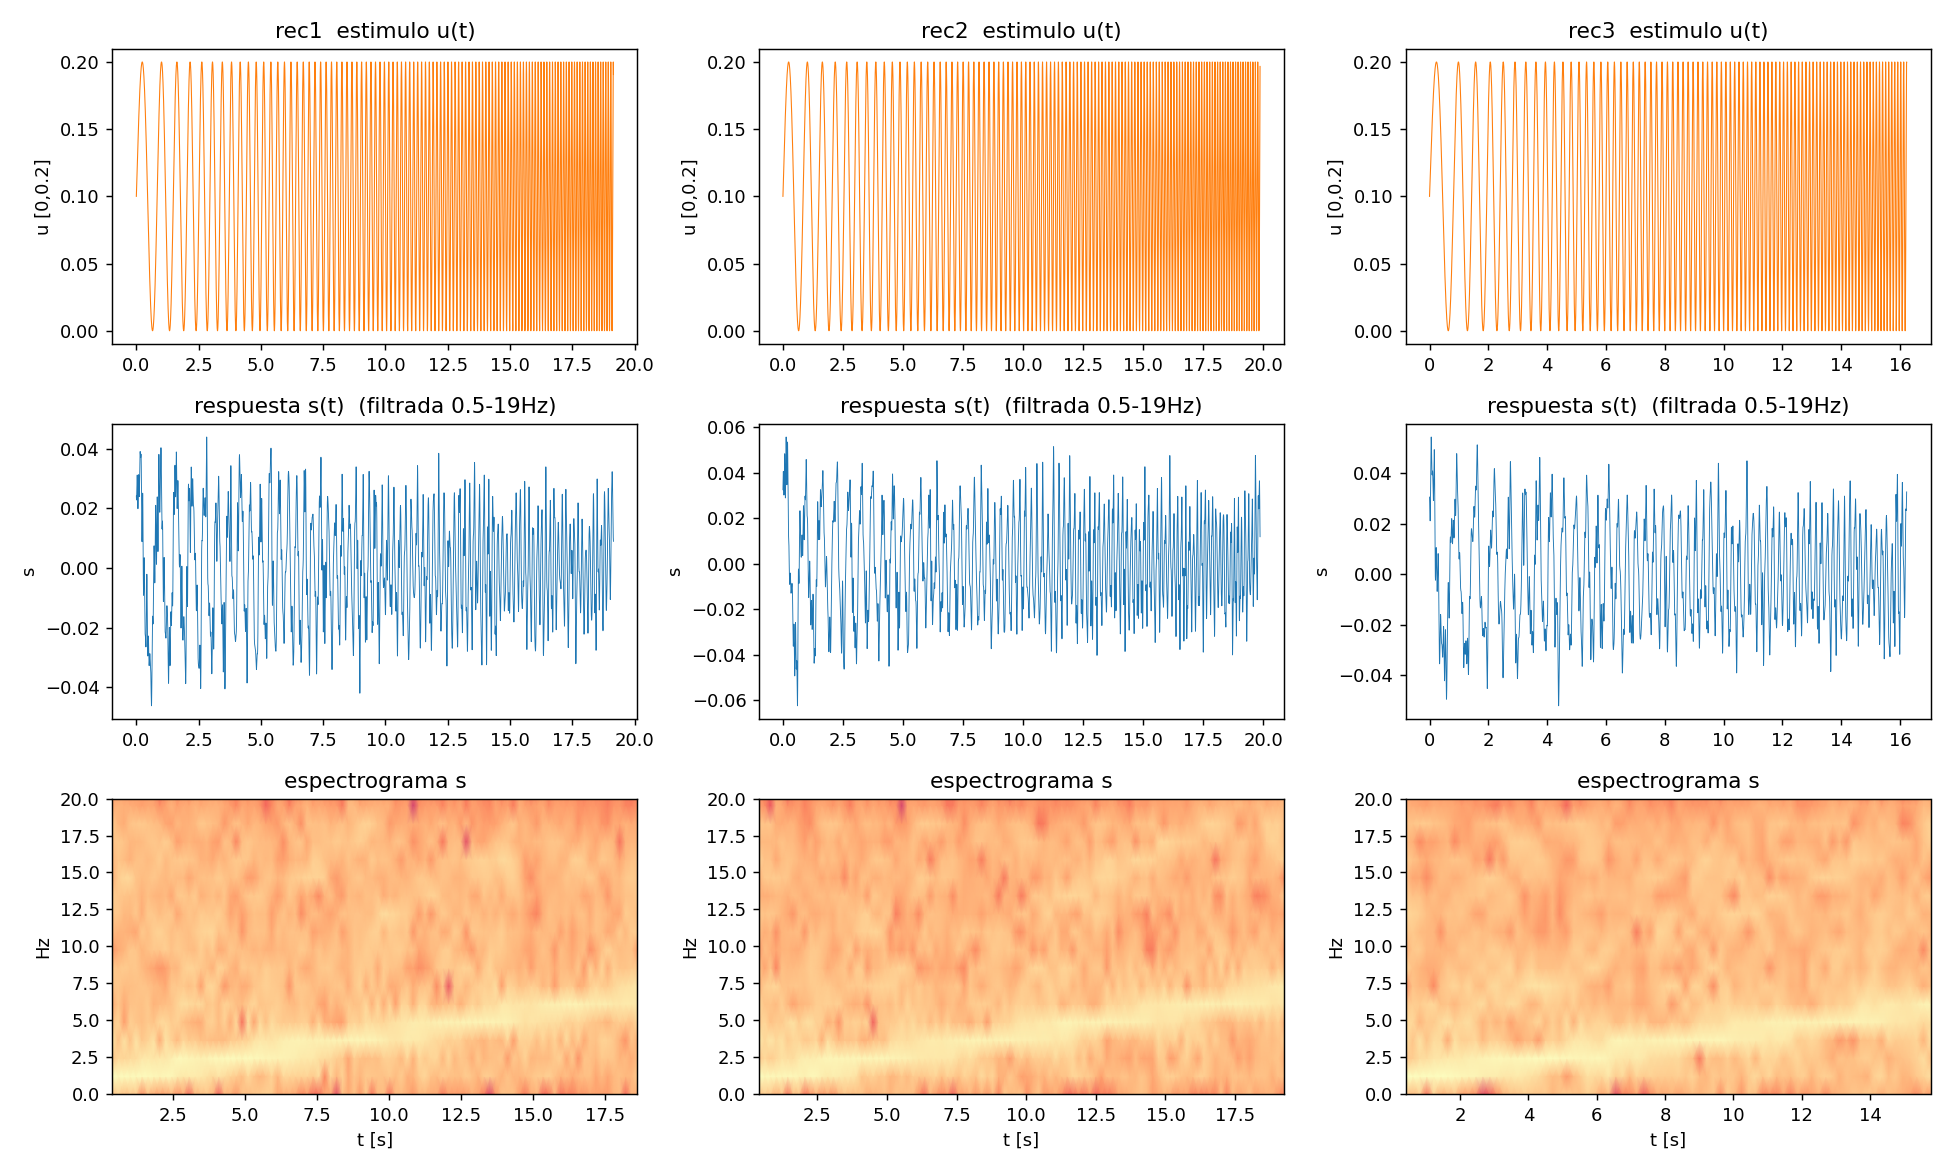
\includegraphics[width=0.85\linewidth]{datos_reales_diagnostico.png}
\caption{Diagnóstico de los datos reales: arriba, $u$ (chirp) y $s$ (LFP filtrada) en el tiempo; abajo, sus espectrogramas. La cresta espectral de la respuesta acompaña la frecuencia instantánea del chirp, evidencia de respuesta forzada. (figura del proyecto)}
\label{fig:diagnostico}
\end{figure}

\subsection*{Conversión a \texttt{.npz}}
El script \texttt{load\_real\_data.py} no identifica nada: solo empaqueta el \texttt{.mat} a un \texttt{.npz} cómodo, con opción de decimar. Los cuidados que importan:
\begin{enumerate}[leftmargin=1.6em]
  \item $u_i, s_i$ son vectores columna $(N,1)$: se aplanan a 1-D con \texttt{ravel}.
  \item \texttt{fsd} es \texttt{uint16}: castear a \texttt{float} antes de dividir.
  \item La \textbf{decimación} usa un anti-alias IIR (Chebyshev, fase cero). Como la banda útil llega a $19$\,Hz, con $f_s^{\text{out}} \ge 250$\,Hz (Nyquist $125$\,Hz) sobra margen. Se generan dos datasets: \texttt{data8\_fs250.npz} ($\times 5$, para producción) y \texttt{data8\_fs125.npz} ($\times 10$, para iterar rápido). El \emph{ringing} del IIR lleva $u$ a $\approx -0.001$; si se necesita $u\ge0$ estricto se decima con FIR o se clipea.
\end{enumerate}
Se trabajó a 125\,Hz para iterar y a 250\,Hz para producción; en ambos el \emph{rollout} de una grabación es de $\sim$2--5\,k pasos, viable con \emph{backprop}.

\section{El problema: identificación por salida}

\subsection*{Ecuaciones y decisiones de modelado}
El modelo es Wilson--Cowan en su forma canónica, con estado $\mathbf{x}=[I,E]$ y sigmoidea $S_a(u)=1/(1+e^{-a u})$:
\begin{align}
\dot I &= \tfrac{1}{\tau_i}\big(-I + S_i(w_{IE}E - w_{II}I + Q(t) - \theta_i) - k_i\big),\\
\dot E &= \tfrac{1}{\tau_e}\big(-E + S_e(w_{EE}E - w_{EI}I + P(t) - \theta_e) - k_e\big),
\end{align}
con $k_e,k_i$ derivados (no aprendidos) para que $E=I=0$ sea el reposo sin estímulo, y salida $y=E-I$. Sobre este esqueleto se toman las decisiones que conectan el modelo con los datos:
\begin{itemize}[leftmargin=1.4em]
  \item \textbf{Entrada:} el estímulo entra a la población excitatoria, $P = c_P\, u$, $Q = 0$, con $c_P$ una ganancia libre (decisión D2).
  \item \textbf{Salida:} $s = c_{\text{out}}\,(E-I)$, con $c_{\text{out}}$ libre y offset $b=0$ (la señal ya viene sin DC porque está pasa-banda; decisión D3).
  \item \textbf{Comparación:} el $\hat y$ simulado se compara en el mismo dominio filtrado $[0.5,19]$\,Hz que $s$, para que el modelo no tenga que "explicar" componentes que fueron filtradas (decisión D4).
\end{itemize}

\subsection*{Por qué esto rompe el pipeline de estado completo}
La diferencia de fondo con los datos sintéticos: allá se medía el estado completo $[I,E]$, así que el \emph{multiple shooting} podía \textbf{resetear} $x_0$ desde el estado observado en cada ventana y comparar contra $[I,E]$ directamente. Con datos reales \textbf{eso no existe}: solo tenemos el escalar $s\approx y$. Consecuencias:
\begin{enumerate}[leftmargin=1.6em]
  \item El estado inicial $[I_0, E_0]$ de cada grabación es \textbf{desconocido}: pasa a ser una variable a estimar.
  \item El \emph{multiple shooting} tal cual no aplica ---no hay estados que resetear. Se pasa a \emph{multiple shooting por salida}: el $x_0$ de \emph{cada ventana} es una \textbf{variable latente} que se optimiza, con una penalización de \textbf{continuidad} que ata el fin de una ventana con el inicio de la siguiente.
  \item Aparece un \textbf{modelo de observación} ($s = c_{\text{out}}(E-I)$) y escalas nuevas que en lo sintético no existían: $c_P$, $c_{\text{out}}$ y la escala de tiempo (absorbida por $\tau_e,\tau_i$ libres).
\end{enumerate}
Esto es identificación de sistemas no lineal \emph{por salida} estándar (\emph{gray-box}), el marco clásico de Ljung~\cite{ljung}. Pero \textbf{no} es lo que corría el repo, así que se escribió un trainer nuevo: \texttt{train\_real\_output.py}. Su núcleo es trocear cada grabación en ventanas cortas ($W$ pasos, $\sim$0.8\,s), rodar la EDO en cada ventana desde su $x_0$ latente, comparar $y$ y $s$ \emph{demediados} por ventana (aproxima el pasa-banda sin filtro global), y sumar un término de continuidad $\lambda_{\text{cont}}\,\|x_0^{(k+1)} - \text{fin}(x^{(k)})\|^2$ que reata las ventanas para que los parámetros WC sigan siendo globales.

\begin{remark}[Por qué ventanas y no un rollout largo]
Un \emph{rollout} de $\sim$2400 pasos ajustado con MSE en el tiempo \textbf{colapsa a salida cero}: si la fase no coincide casi exacto, predecir $0$ tiene \emph{menos} error que una oscilación desfasada, y el gradiente cae al mínimo trivial. Cortar en ventanas cortas hace la fase local (tratable), batchea (mucho más rápido), y la continuidad recompone el todo.
\end{remark}

\section{Validación por partes}
Antes de invertir en el pipeline WC completo se validaron los supuestos con experimentos baratos, de menor a mayor compromiso.

\subsection{Coherencia $u\to s$}
La coherencia espectral entre $u$ y $s$ (estimador de Welch) es \textbf{alta a baja frecuencia}: pico $\approx 0.96$ a $\sim$1.7\,Hz, y decae al subir. Como el chirp es no estacionario, la coherencia de Welch está sesgada, pero el mensaje es robusto: \textbf{hay relación entrada--salida}, coincidente con lo que muestra el espectrograma (fig.~\ref{fig:diagnostico}).

\subsection{Baseline ARX (modelo lineal)}
El techo lineal se estima con un \textbf{ARX} (auto-regresivo con entrada exógena, órdenes $n_a$ para el pasado de $s$ y $n_b$ para el de $u$), ajustado por mínimos cuadrados:

\begin{table}[H]
\centering
\small
\begin{tabular}{@{}lcc@{}}
\toprule
orden $(n_a, n_b)$ & $R^2$ \emph{teacher-forcing} (in-sample) & $R^2$ cruzado (fit rec0 $\to$ rec1/2) \\
\midrule
$(0, 40)$ --- solo FIR de $u$ & $0.14$ & $0.10$ \\
$(2, 20)$ & $\mathbf{0.987}$ & $\mathbf{0.987 / 0.988}$ \\
$(4, 40)$ & $\sim\!1.00$ & $0.998 / 0.999$ \\
\bottomrule
\end{tabular}
\caption{ARX en modo \emph{teacher-forcing} (predicción a 1 paso). El $R^2\approx0.99$ y su reproducibilidad \emph{cruzada} sugieren un ajuste inmejorable... pero ese número usa el pasado \emph{real} de $s$.}
\label{tab:arx}
\end{table}

A primera vista parece cerrado: $R^2\approx0.99$, y el ajuste \textbf{cruzado} (parámetros de la grabación 0 aplicados a las otras) es casi idéntico $\Rightarrow$ los parámetros son \textbf{reproducibles entre grabaciones}. La trampa está en que ese $R^2$ es \textbf{predicción a un paso}: en cada instante usa el valor \emph{medido} de $s$ un instante antes. Es exactamente la letra chica que separa este documento en dos.

\section{El hallazgo central: predicción vs.\ simulación libre}

\subsection*{El experimento decisivo}
Tomemos el \textbf{mismo} ARX de la tabla~\ref{tab:arx} y corrámoslo en \textbf{simulación libre}: solo con $u$, realimentando su \emph{propia} salida (que es exactamente lo que hace un \emph{rollout} de Wilson--Cowan). El contraste es brutal:

\begin{table}[H]
\centering
\small
\begin{tabular}{@{}lc@{}}
\toprule
modo & $R^2$ \\
\midrule
\emph{teacher-forcing} (predicción 1 paso, usa el pasado real de $s$) & $\mathbf{0.99\text{--}1.00}$ \\
\textbf{simulación libre} (solo $u$, realimenta su salida) & $\mathbf{0.04\text{--}0.11}$ \\
\bottomrule
\end{tabular}
\caption{El mismo modelo, dos métricas. La predicción a 1 paso "calca" $s$; la simulación libre apenas llega a $R^2\sim0.1$.}
\label{tab:pred_vs_sim}
\end{table}

La figura~\ref{fig:hallazgo} lo muestra crudo: arriba, la predicción a un paso se \emph{superpone} a $s$; abajo, la simulación libre produce una oscilación limpia con la frecuencia correcta pero \textbf{desfasada y sin la estructura fina} de $s$.

\begin{figure}[H]
\centering
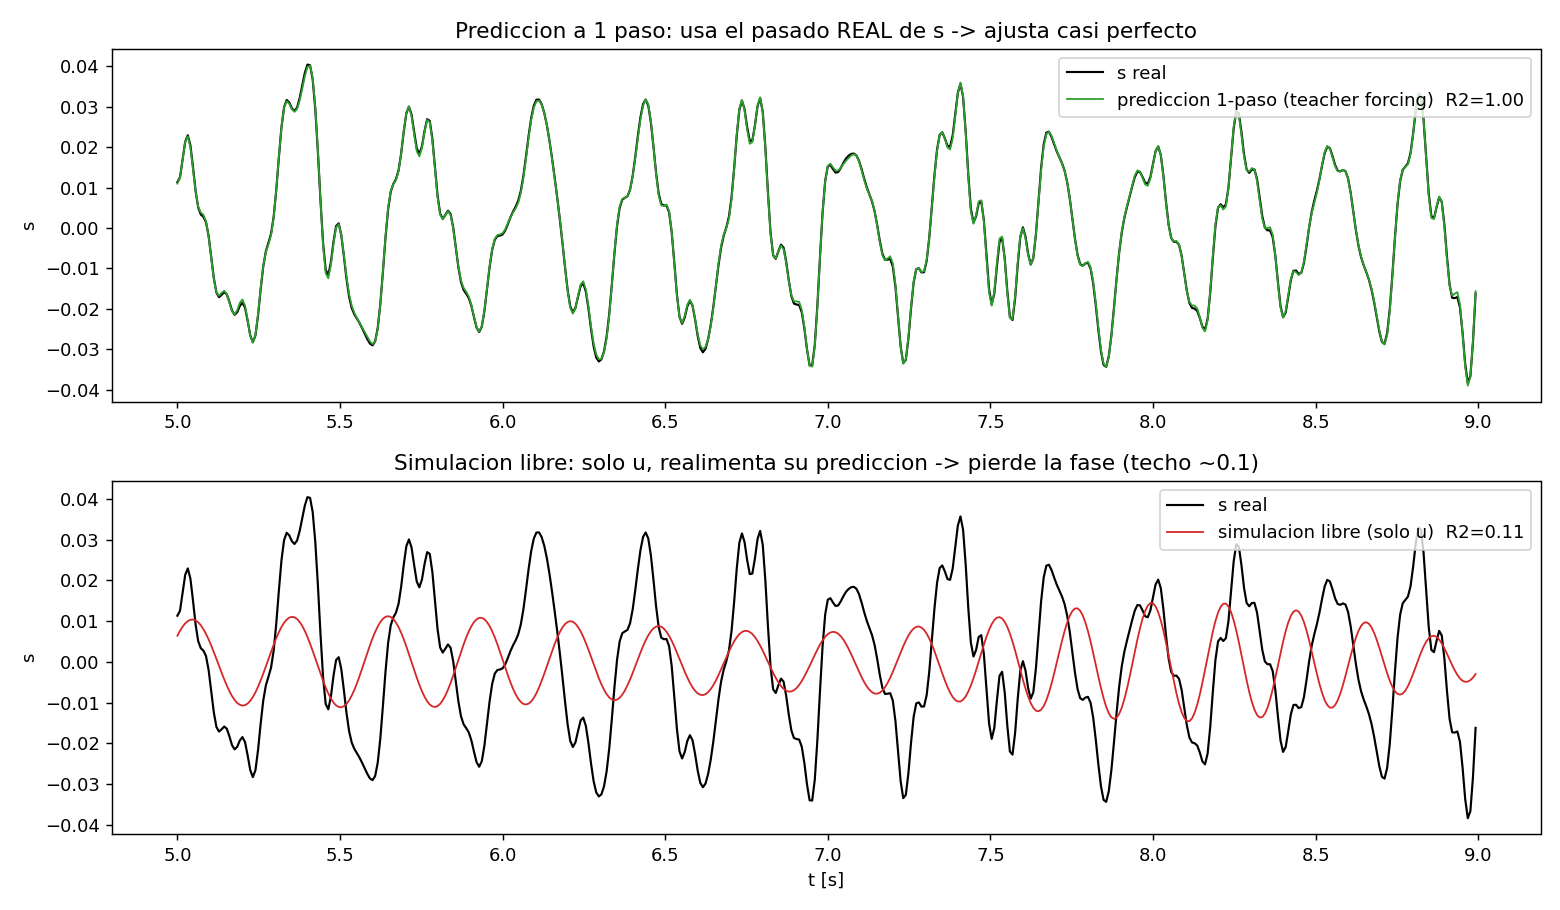
\includegraphics[width=0.85\linewidth]{real_teacherforcing_vs_simlibre.png}
\caption{\textbf{El hallazgo central.} Arriba: predicción a 1 paso (\emph{teacher-forcing}) sobre $s$; el modelo calca la señal ($R^2\approx0.99$). Abajo: simulación libre desde $u$; oscilación con la frecuencia correcta pero desfasada, $R^2\approx0.1$. La brecha entre ambas mide cuánto de $s$ gobierna $u$. (figura del proyecto)}
\label{fig:hallazgo}
\end{figure}

\subsection*{Qué significa}
\begin{quote}
El estímulo $u$ explica solo $\sim$\textbf{10\,\%} de la varianza de $s$ en modo simulación. El resto lo hace la \textbf{dinámica interna/estocástica} del sistema.
\end{quote}
La evidencia complementaria: sin la parte auto-regresiva ($n_a=0$, solo FIR de $u$) el $R^2$ cae a $0.14$ (tabla~\ref{tab:arx}, primera fila). Es decir, la parte que "usa el pasado de $s$" ---la dinámica recurrente--- hace casi todo el trabajo; $u$ sola aporta poco.

\subsection*{El WC en las dos métricas}
Con el trainer por salida (multiple shooting, estado latente por ventana), Wilson--Cowan se comporta según qué métrica se le exija:

\begin{table}[H]
\centering
\small
\begin{tabular}{@{}lcl@{}}
\toprule
métrica & $R^2$ WC & comentario \\
\midrule
predicción a horizonte corto (ventana $\sim$16 pasos $=128$\,ms) & $\mathbf{\approx 0.85}$ & la dinámica WC \emph{sí} es identificable \\
\emph{rollout} libre de toda la traza (solo $u$) & $\approx 0.01\text{--}0.05$ & cerca del techo real ($\sim0.1$) \\
\bottomrule
\end{tabular}
\caption{WC identificado por salida. En el marco correcto (predicción a horizonte corto) alcanza $R^2\approx0.85$; en \emph{rollout} libre queda cerca del techo real de la tarea.}
\label{tab:wc}
\end{table}

La lectura clave: el WC en \emph{rollout} libre daba $\sim$0 \textbf{porque la tarea tiene techo $\sim$0.1}, no porque el trainer o la hipótesis $u\to E$ estuvieran mal. \textbf{No es un fallo del modelo: es una propiedad medible de los datos.}

\section{Por qué el \emph{rollout} libre "no anda" (y por qué está bien)}
Tres cosas se confundieron al principio; conviene separarlas:
\begin{enumerate}[leftmargin=1.6em]
  \item \textbf{Colapso a salida cero.} Ajustar una señal oscilatoria con MSE en el tiempo, si la fase no calza casi exacto, premia "predecir 0" por sobre una oscilación desfasada $\Rightarrow$ mínimo trivial. Se mitiga con una \emph{loss} normalizada / de correlación y con las ventanas cortas.
  \item \textbf{Degeneración con estado latente.} Ventanas cortas $+$ $x_0$ latente ajustan \emph{localmente} incluso con un modelo inestable o incorrecto (los resets enmascaran la inestabilidad); el \emph{rollout} libre después diverge. Se mitiga con continuidad fuerte, regularización de parámetros y \emph{curriculum} de longitud de ventana.
  \item \textbf{El techo real.} Aun arreglando 1 y 2, la simulación libre desde $u$ no puede pasar de $R^2\sim0.1$ \textbf{porque $u$ no gobierna a $s$}. Esto lo confirma el ARX (tabla~\ref{tab:pred_vs_sim}): no es un problema numérico, es la física de los datos.
\end{enumerate}
El punto 3 es el que hay que internalizar: un techo bajo en simulación libre es un \emph{dato del experimento} (input débil), no un veredicto sobre el modelo.

\section{Implicaciones para los dos protocolos}
El proyecto pidió dos protocolos de validación. El hallazgo reordena las expectativas:
\begin{itemize}[leftmargin=1.4em]
  \item \textbf{Protocolo A --- generalización entre trayectorias (leave-one-out).} \emph{Viable} en modo predicción. Se ajusta un solo juego de parámetros sobre 2 grabaciones y se mide en la tercera, rotando. El techo cruzado es $\approx0.99$ y los parámetros son reproducibles entre las 3 grabaciones. Es el protocolo \textbf{fuerte} para estos datos.
  \item \textbf{Protocolo B --- continuación temporal (forecast por rollout libre).} \emph{Limitado} por el techo de simulación ($\sim0.1$). "Continuar la trayectoria" desde $u$ solo no es alcanzable con alta precisión: es propiedad de los datos, no del modelo. La métrica \emph{honesta} de forecast es a \textbf{horizonte corto} (predecir los próximos $k$ pasos dado el pasado reciente), no continuación indefinida.
\end{itemize}
Nada de esto invalida el objetivo: la identificación paramétrica se hace en \textbf{modo predicción}, que es el marco estándar (\emph{prediction-error method}~\cite{ljung}). Lo que cambia es el criterio de éxito y la expectativa sobre el \emph{rollout} libre.

\section{Conexión con la teoría de identificabilidad}
Que $u$ sea un \emph{driver} débil y que el régimen sea \textbf{casi lineal de 2\textsuperscript{o} orden} tiene una consecuencia directa sobre la identificabilidad. De los 10 parámetros de WC, los datos solo restringen $\sim$4--5 \textbf{combinaciones efectivas}: los 2 polos de la dinámica linealizada más las ganancias $c_P, c_{\text{out}}$. El resto de las direcciones en el espacio de parámetros queda \textbf{sin excitar}.

En el lenguaje del proyecto: habrá \textbf{direcciones planas} en la Matriz de Información de Fisher (FIM) del ajuste real, exactamente el fenómeno de mal condicionamiento que se analiza con SVD y se acota con Cramér--Rao (ver M6). El input débil es una fuente de no identificabilidad \emph{práctica} adicional a la estructural: aunque la parametrización fuera perfecta, un estímulo que aporta $\sim$10\,\% de la varianza no puede tensar todas las direcciones del modelo. Es la contracara concreta de por qué el diseño de experimentos (excitación persistente, amplitud de estímulo) importa tanto en identificación~\cite{ljung, raue}. El análisis FIM/SVD sobre el óptimo \emph{real} ---no ya sintético--- es por lo tanto parte central del entregable, y se espera que \emph{muestre y explique} la baja identificabilidad de varios parámetros.

\section{Estado y próximos pasos}
\textbf{Hecho y validado:}
\begin{itemize}[leftmargin=1.4em, itemsep=1pt]
  \item Conversión y verificación del \texttt{.mat}; datasets \texttt{data8\_fs\{250,125\}.npz}.
  \item Diagnóstico espectral $+$ coherencia $u\to s$.
  \item Baseline ARX (predicción y simulación) y el hallazgo predicción-vs-simulación.
  \item Trainer por salida (\texttt{train\_real\_output.py}) con multiple shooting y estado latente.
  \item WC identificable a horizonte corto ($R^2\approx0.85$); \emph{rollout} libre cerca del techo $\sim$0.1.
\end{itemize}

\textbf{Abierto:}
\begin{enumerate}[leftmargin=1.6em, itemsep=1pt]
  \item \textbf{Reencuadrar el trainer al marco de predicción a $k$ pasos} (\emph{prediction-error}): optimizar predicciones de horizonte corto y reportar $R^2$ \emph{vs.}\ horizonte (la curva que va de \emph{teacher-forcing} a simulación) como métrica principal.
  \item \textbf{Inicialización principista:} anclar la WC linealizada a los \textbf{polos del ARX orden-2} $\Rightarrow$ arranque bien condicionado.
  \item \textbf{Protocolo A completo} (leave-one-out en modo predicción, 3 folds) con barras de parámetros y su dispersión.
  \item \textbf{V1 (gray-box):} ver si la corrección $g_\phi$ captura parte de la dinámica intrínseca que $u$ no explica, cuidando que \emph{no "tape"} al WC (que la parte WC siga interpretable). Como $s$ no está gobernada por $u$, $g_\phi$ sin entrada no puede inventar la estocástica; su rol es corregir la estructura, no predecir el ruido.
  \item \textbf{FIM/SVD} sobre el óptimo real $\Rightarrow$ identificabilidad e incertidumbre (Cramér--Rao).
\end{enumerate}

\begin{remark}[La moraleja]
El entregable más valioso de esta tanda no es un $R^2$ sino un \emph{diagnóstico}: aprendimos que el estímulo disponible es un \emph{driver} débil, que la identificación debe hacerse en modo predicción, y que el techo del \emph{rollout} libre es una propiedad del experimento. Un resultado negativo bien caracterizado vale más que un ajuste optimista mal entendido.
\end{remark}

\begin{thebibliography}{9}
\bibitem{ljung} L. Ljung, \emph{System Identification: Theory for the User}, 2\textsuperscript{a} ed., Prentice Hall, 1999.
\bibitem{raue} A. Raue et al., ``Structural and practical identifiability analysis of partially observed dynamical models by exploiting the profile likelihood'', \emph{Bioinformatics} 25(15):1923--1929, 2009.
\bibitem{wc1972} H. R. Wilson y J. D. Cowan, ``Excitatory and inhibitory interactions in localized populations of model neurons'', \emph{Biophysical Journal} 12(1):1--24, 1972.
\end{thebibliography}

\end{document}
